\subsubsection*{Rede neural profunda}

A principal diferença entre uma rede neural artificial e uma rede neural profunda é a quantidade de camadas, uma rede neural profunda possui várias camadas de processamento \apud{marti2017aprendizado}{haykin1999neural}.

\begin{figure}[ht]
	\centering
	\caption{Comparação de uma rede neural convencional com uma rede neural profunda.}
	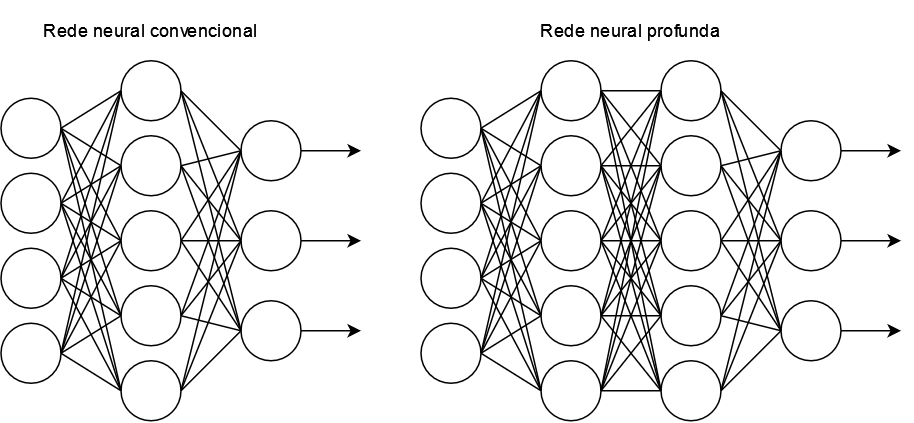
\includegraphics[width=0.8\textwidth]{figures/redes_neurais.png}
	\legend{Fonte: Criação própria}
	\label{fig:redes_neurais}
\end{figure}